\documentclass{article}
\usepackage[tmargin=1in, bmargin=1in, lmargin=1.2in, rmargin=1.2in]{geometry}
%%% Sets numbering depth to subsection level (e.g, no numbered subsubsections)
\setcounter{secnumdepth}{2}

\usepackage{macrosabound, theorem-env}
\usepackage[shortlabels]{enumitem}

%%%%%%%%%%%%%%%%%%%%%%%%%%%%%%%%%%%%%%%%%%
%%% TIKZ SETUP FOR FLOWCHARTS
%%%%%%%%%%%%%%%%%%%%%%%%%%%%%%%%%%%%%%%%%%
\usetikzlibrary{shapes.geometric, arrows}
\tikzstyle{startstop} = [rectangle, rounded corners, 
minimum height=1cm,
minimum width=2cm,
text centered, 
draw=black, 
fill=red!30]

% tikzstyle stuff
\tikzstyle{io} = [trapezium, 
trapezium stretches=true, % A later addition
trapezium left angle=70, 
trapezium right angle=110, 
minimum height=1cm, text centered, 
draw=black, fill=blue!30]

\tikzstyle{process} = [rectangle,
minimum height=1cm, 
text centered, 
align=center,
draw=black, 
fill=orange!30]

\tikzstyle{decision} = [rectangle, rounded corners,
minimum height=1cm, 
text centered, 
align=center,
draw=black, 
fill=green!30]
\tikzstyle{arrow} = [thick,->,>=stealth]

% make font smaller
\usepackage[fontsize=10pt]{fontsize}%%% Coloring the comment as blue

% algorithms
\usepackage[linesnumbered,ruled,vlined]{algorithm2e}
\newcommand\mycommfont[1]{\footnotesize\ttfamily\textcolor{blue}{#1}}
\SetCommentSty{mycommfont}
\SetKwInput{KwInput}{Input}                % Set the Input
\SetKwInput{KwOutput}{Output}              % set the Output

%%%%%%%%%%%%%%%%%%
%%%% FOR DEBUGGING
%%%%%%%%%%%%%%%%%%
%\usepackage{layout}
%\usepackage{showframe}

%%% Removes paragraph indentation and changes paragraph line skip

% ensures that the references show up as an unnumbered section
\def\bibsection{\section*{\refname}} 
\begin{document}
%%% The Title and Author only need to be set once at the start of the document. If you take notes for multiple courses in the same document (for example, in a multi-semester sequence for the same course), you can separate the courses with a new Part, and the semester, lecturer, and course only need to be set once at the start of the new course.
\newpage
\title{The Reverse Ising Problem}
\author{Isaac Martin and Andrew Moore}
\date{Summer 2023}
\maketitle
\tableofcontents
\section{Foundations}

\subsection{Circuits}
Throughout this document we set $\Sigma = \{-1,1\}$ to be the set of possible spins ($\Sigma$ for \textbf{s}pin) taken by a single vertex in an Ising graph. For any set $X$, we denote by $\Sigma^X$ the set of all functions $\sigma: X\to \Sigma$ and note, by setting $n = |X|$, that $\Sigma^X$ can equivalently be viewed as the set of $n$-tuples valued in $\{-1, 1\}$, $\Sigma^X \cong \{(\sigma_1, ..., \sigma_n) \in \Sigma^n \}$ or as the set of binary strings of length $n$ under the identification $\Sigma \leftrightarrow \{0,1\}$. We first review a few elementary facts.

\begin{prop}Let $X$ be any set.
  \begin{enumerate}[(a)]
    \item If $\alpha:N \hookrightarrow X$ then we have a map $\res_{XN}\Sigma^X \to \Sigma^N$ given $\res_{XN}(\sigma) = \sigma \circ \alpha.$ We denote $\res_{XN}(\sigma) = \sigma|_N$.
  \item If $N, M \subseteq X$ are disjoint, then $\Sigma^N \times \Sigma^M \cong \Sigma^{N \cup M}$. em
  \item If $N, M \subseteq X$ are not necessarily disjoint, then $\Sigma^N \times_{N\cap M} \Sigma^M \cong \Sigma^{N\cup M}$.
  \end{enumerate}
\end{prop}
\begin{proof}$ $
  \begin{enumerate}[(a)]
    \item Trivial; statement of fact.
    \item This is a special case of (c).
    \item The object $\Sigma^{N\cup M}$ fits into the following diagram
      \begin{center}
        \begin{tikzcd}
          \Sigma^{N\cup M} \arrow[r, "\res"] \arrow[d, "\res"] & \Sigma^N \arrow[d, "\res"] \\
          \Sigma^M \arrow[r, "\res"] & \Sigma^{N\cap M}
        \end{tikzcd}
      \end{center}
      where all maps are the appropriate restriction maps. In fact, $\Sigma^{N\cup M}$ together with restriction maps is the universal object of this diagram; suppose we have another object $P$ with maps $q_1:P \to \Sigma^M$ and $q_2:P\to \Sigma^N$ making this commute. Then $\res(q_1(p)) = \res(q_2(p))$ so the map $u: P\to \Sigma^{N\cup M}$ given by
      \begin{align*}
        u(p)(x) =
        \begin{cases}
          q_1(p)(x) & x \in M \\
          q_2(p)(x) & x \in N
        \end{cases}
      \end{align*}
      is well defined on $M\cap N$. Hence $\Sigma^{N\cup M}$ is the pullback of $\Sigma^M$ and $\Sigma^N$ with restriction maps to $\Sigma^{N\cap M}$.
  \end{enumerate}
\end{proof}


\begin{defn}\label{defn:abstract-circuit}
  A \textbf{circuit} is a tuple $(N, M, f)$ where
  \begin{itemize}
    \item $N, M \subseteq X$ are arbitrary subsets of some universal set $X$ and are almost always chosen so that $N \cap M = \emptyset$. Both $N$ and $M$ should be finite and we call their elements \textbf{input} and \textbf{output} spins respectively.
    \item $f: \Sigma^N \to \Sigma^M$ is an arbitrary function called the \emph{logic} function.
  \end{itemize}
  We make special note of the scenarios in which $N$ and $M$ are not disjoint. Additionally, we define the following terminology.
  \begin{itemize}
    \item $A = X \setminus (N\cup M)$ is the \textbf{set of auxiliary spins} of $X$.
    \item $\Sigma^X$ is the \textbf{spin space}, $\Sigma^N$ is the \textbf{input space}, $\Sigma^M$ the \textbf{output space} and $\Sigma^N$ the \textbf{auxiliary space} of $X$. Elements of $\Sigma^X$ are called \textbf{spin states}, elements of $\Sigma^N$ \textbf{input states}, etc.
    \item $\cR(f) = \{\sigma \in \Sigma^X \mid f(\sigma|_N) = \sigma|_M\}$ is the set of \textbf{correct} or \textbf{right} spin states.
    \item $\cW(f) = \Sigma^X \setminus \cR(f)$ is the set of \textbf{wrong} spin states.
    \item $\cL(\sigma) = \cL(\sigma|_N) = \{\sigma' \in \Sigma^X \mid \sigma'|_N = \sigma|_N\}$ is the \textbf{input level} of $\sigma$. It is useful to talk about the input level of both an input state $\sigma|_N$ and a full spin state $\sigma$, so we write $\cL(\sigma)$ and $\cL(\sigma|_N)$ to mean the same thing.
  \end{itemize}
\end{defn}

At this point it is worth remarking that this object $(N,M,f)$ in no way carries the data of an Ising system. An Ising system is a collection of spins with connections between them, together with a fixed quadratic Hamiltonian which predicts the dynamics of the system. What we have defined has no Hamiltonian, no notion of dynamics and no real semblance of a graph structure; it has only a function which specifies a desired output to each input and a lot of extra space ($X\setminus (N\cup M)$ with which to begin adding additional structure. An abstract circuit, as defined, is nothing other than a skeleton for an Ising system we wish to design. 

\subsection{The Reverse Ising Problem}

\begin{defn}\label{defn:ising-system}
  An \textbf{Ising system} is a pair $(X, H)$, often referred to as simply $X$, where
  \begin{itemize}
    \item $X \subseteq \bN$ is a set whose elements are called \textbf{spins},
    \item $H \in \bR[X]$ is a quadratic polynomial called the \emph{Hamiltonian} of $X$.
  \end{itemize}
  The \textbf{state space} of $X$ is $\Sigma^X$. An Ising system $X$ in state $\sigma \in \Sigma^X$ has energy $H(\sigma)$ given by evaluating the Hamiltonian at $\sigma$.
\end{defn}

An Ising system is inherently probabilistic. The probability that an Ising system $X$ is in state $\sigma \in \Sigma^X$ is given by the \textbf{configuration probability}
\begin{align*}
  P_\beta = \frac{e^{-\beta H(\sigma)}}{Z_\beta}
\end{align*}
where $\beta = (k_BT)^{-1} \geq 0$ is inverse temperature, $k_B$ is the Boltzmann constant and the normalization constant $Z_\beta$ is the partition function $Z_\beta = \sum_{\sigma \in \Sigma^X} e^{-\beta H(\sigma)}$. Notice that probability is maximized whenever the Hamiltonian is minimized, hence low energy states are more probable than high energy states.

With this in mind, for an Ising system with $(X,H)$ with $X$ finite and a subset $U \subseteq X$, we define the \textbf{minimizer with respect to $U$} to be the function $m_U: \Sigma^U \to \Sigma^{X}$ defined
\begin{align*}
f_U(\tau) = \argmin_{\sigma \in \Sigma^X, ~\sigma|_U = \tau} H(\sigma).
\end{align*}
It answers the question: ``if the states of $U$ are held fixed, then what is the most likely state of $X$?'' We likewise define the \textbf{minimizer logic} of $U$ to be the function $f_U:\Sigma^U \to \Sigma^{U^c}$ given $f_U(\tau) = m_U(\tau)|_{U^c}$.

\bigskip

We would like to design Ising systems with the following features:
\begin{enumerate}[(1)]
  \item A subset $N \subseteq X$ of spins whose state can be fixed
  \item A subset $M \subseteq X$ whose states vary freely with dynamics
  \item For a choice $\sigma_N \in \Sigma^N$, the most likely spin state in $\sigma_M \in \Sigma^M$ is $f(\sigma_N)$, where $f: \Sigma^N \to \Sigma^M$ is some function.
\end{enumerate}
Stated another way, given an abstract circuit $(N,M,f)$, we want to design Ising systems such that for every choice of input state $\sigma|_N$, the state $\sigma'$ which minimizes energy among all states matching $\sigma$ in input is a correct spin state. That is,
\begin{align*}
  \argmin_{\sigma' \in \cL(\sigma)} H(\sigma') \in \cR(f) ~ \text{ for all } ~ \sigma \in \Sigma^X.
\end{align*}

\begin{defn}\label{defn:solves-ising-circuit}
  Fix an abstract circuit $(N, M, f)$. We say that an Ising system $(X, H)$ \textbf{solves} $(N, M, f)$ (in that it solves the reverse Ising problem on $(N,M,f)$) if for each $\sigma \in \Sigma^X$ 
  \begin{align*}
    \tau = \argmin_{\sigma' \in \cL(\sigma)} ~H(\sigma') \implies \tau \in \cR(f).
  \end{align*}
  In other words, a choice of Hamiltonian $H$ for $X$ solves the circuit if the minimizer of the Hamiltonian among all states with matching input states has as its output component the correct output as specified by the circuit logic $f$.

  An \textbf{Ising circuit} is an abstract circuit $(N,M,f)$ with $N,M \subset X$ together with an Ising system $(X,H)$ such that $(X,H)$ solves $(N,M,f)$.
\end{defn}

\subsection{Constraint Sets for Designing Ising Systems}
Let us first consider the simplest case of a circuit $(N, M, f)$ with $X = N \cup M$ and $N$ and $M$ disjoint.
\begin{lem}\label{lem:basic_constraints}
  The circuit $X$ is solvable with an Ising system if and only if there exists a Hamiltonian $H$ such that for all $s\in \Sigma^N$ and $t \neq f(s)$ $H(s,t) > H(s,f(s))$.
\end{lem}
\begin{proof}
  Obvious, is essentially the definition of the Ising system solvability.
\end{proof}
It is not hard to find examples of circuits which are not solvable, for instance, the naive XOR circuit with $|X| = 3$ is not solvable with an Ising system.

For the remainder of this section, suppose that $X = N \cup M \cup A$ is a finite set and $N$, $M$, and $A$ are all disjoint. We call elements of this extra set $A$ \textbf{auxiliary spins}.

\begin{prop}\label{prop:can_solve_with_aux}
  Let $X \subseteq \bN$ be infinite and $N$, $M$ be finite disjoint subsets. For any choice of $f$, the circuit $(N, M, f)$ is solvable with an Ising system. Since $|X| > |N\cup M|$ in this case, we sometimes say that $X$ is \textbf{solvable with auxiliary spins}.
\end{prop}
Notice that this lemma says nothing about the \emph{number} of auxiliary spins needed to solve a circuit; in general, it can be quite large.
\begin{proof}
  Take the hamming objective function $\text{ham}:\Sigma^{N\cup M} \to \bR$ defined to be the hamming distance from $\sigma$ to the (unique) correct spin state whose $N$ coordinates match those of $\sigma$:
  \begin{align*}
    \text{ham}(\sigma) = d(\sigma_M, f(\sigma_N)).
  \end{align*}
This has minimum value $0$ obtained precisely at spins with correct output coordinates. It is also a pseudo-boolean function and hence can be written uniquely as a multilinear polynomial. Add auxiliary variables until the degree of this polynomial is $2$ using, for instance, Rosenberg reduction. The obtained quadratic will be an Ising Hamiltonian in $|N \cup M \cup A|$ variables where $A$ is the set of auxiliary variables added during the reduction step. 
\end{proof}

The task of finding an Ising system which solves some abstract circuit $(N, M, f)$ can thus be thought of as finding a sufficiently large cardinality for $A$ and then solving a mixed non-linear optimization problem to find valid a valid quadratic Hamiltonian together with auxiliary states which occur at the desired minimizers of input levels. The following lemma demonstrates one way one might attempt to solve an abstract circuit with auxiliaries. 

\begin{lem}\label{lem:weak_constraints}
  The circuit $(N,M,f)$ is solvable with an Ising system if and only if there exists a function $g:\Sigma^N \to \Sigma^A$ and a Hamiltonian $H$ such that for all $\sigma \in \Sigma^N$, $\eta \in \Sigma^A$ and $f(\sigma) \neq \omega \in \Sigma^M$, $H(\sigma, \omega, \eta) > H(\sigma, f(\sigma), g(\sigma))$.
\end{lem}
The image of the function $g$ is called the \textbf{auxiliary array} of $X$. If we fix a specific spin $a \in A$, then the set $\{g(\sigma)_a\}_{\sigma \in \Sigma^N}$ is called the \emph{auxiliary vector of $a$}.
\begin{proof}
  Again, obvious.
\end{proof}

A solution to a circuit employing Lemma \ref{lem:weak_constraints} consists of two parts: obtaining a feasible auxiliary array $g$ and identifying choices of Hamiltonians such that the constraints in Lemma \ref{lem:weak_constraints} are all satisfied. Although it is always possible, choosing a feasible $g$ is quite difficult, and doing so in such a way that minimizes the cardinality of $A$ is even harder. If a feasible $g$ is known, solving for $H$ is a linear programming problem; however, because the number of constraints in Lemma \ref{lem:weak_constraints} grows exponentially in $N$, $M$ and $A$, for problems on the order of $|X| \approx 100$ there is no computer on earth that can actually solve the LP-problem as stated.

\begin{defn}[Constraint Sets for Reverse Ising]\label{defn:constraints}
  Let $(N,M,f)$ be an abstract circuit with $X = N \cup M \cup A$ and $N, M, A$ all disjoint. We say that an Ising system $(X, H)$ together with a choice $g: \Sigma^N\to \Sigma^A$ of auxiliary array satisfies
  \begin{itemize}
    \item \textbf{Weak Constraints} if for all $\sigma_N \in \Sigma^N$ and $\sigma_M \neq f(\sigma_N)$
      \begin{align*}
        H(\sigma_N, \sigma_M, \sigma_A) > H(\sigma_N, f(\sigma_N), g(\sigma_N)).
      \end{align*}
      There are $2^{M + A} - 2^A$ constraints per input level, $2^N(2^{M+A} - 2^A)$ total.
    \item \textbf{Full Constraints} if for all $\sigma_N \in \Sigma^N$ and $\sigma_M \neq f(\sigma_N)$ \emph{or} $\sigma_A \neq g(\sigma_N)$
      \begin{align*}
        H(\sigma_N, \sigma_M, \sigma_A) > H(\sigma_N, f(\sigma_N), g(\sigma_N)).
      \end{align*}
      There are $2^{M+A} - 1$ constraints per input level, $2^N(2^{M+A} - 1)$ total.
    \item \textbf{$\bfF$-Augmented Constraints} if for some function $F:\Sigma^{N} \times \Sigma^M \to \Sigma^A$
      \begin{align*}
        H(\sigma_N, \sigma_M, F(\sigma_N, \sigma_M)) > H(\sigma_N, f(\sigma_N), F(\sigma_N, f(\sigma_N))).
      \end{align*}
      There are $2^M - 1$ constraints per input level or $2^N(2^M - 1)$ constraints total.
  \end{itemize}
\end{defn}


\begin{lem}\label{lem:full_constraints}
  Let $(N, M, f)$ be an abstract circuit with $X = N \cup M \cup A$ and all $N, M$ and $A$ disjoint. This circuit is solved by an Ising system $(X, H)$ if and only if there is an auxiliary array $g:\Sigma^N \to \Sigma^A$ such that $H$ satisfies full constraints.
\end{lem}
\begin{proof}
  The reverse implication is clear, as every constraint in Lemma \ref{lem:weak_constraints} is a constraint in Lemma \ref{lem:full_constraints}. 

  For the forward implication, suppose $(N,M,f)$ is solved by an Ising system $(X,H)$. Defining $g$ to be the auxiliary component of the minimizer with respect to $N$, $g(\sigma_N) = m_N(\sigma_N)|_{A}$, does the trick.
\end{proof}

The next lemma addresses the use of the $F$-augmented constraints, and is the most useful result in this section. It is the primary result underpinning the authors' approach to the reverse Ising problem.
\begin{lem}\label{lem:augmented_constraints}
  Let $(N, M, f)$ again be an abstract circuit. There exists an Ising system which solves this circuit if and only if there is some function $F:\Sigma^N\times\Sigma^M \to \Sigma^A$ such that both
  \begin{enumerate}[(a)]
    \item the new circuit $(N\cup M, A, F)$ is solvable by an Ising system with Hamiltonian $R$ with the following additional property:
      \begin{equation}\label{eqn:weak-neutralizability}\tag{$\dagger$}
        R(\sigma_N, \sigma_M, F(\sigma_N,\sigma_M)) \geq R(\sigma_N, f(\sigma_N), F(\sigma_N, f(\sigma_N)))
      \end{equation}
      for all $\sigma_N$ and $\sigma_M$. We call this the \textbf{weak neutralizability condition.} (If the inequality is instead an equality, we call this the \textbf{strong neutralizability condition.} Likewise, if such an Ising system (X,R) exists, we correspondingly say that $F$ is weakly neutralizable or strongly neutralizable.) We call the system $(X, R)$ the \textbf{auxiliary system} and the circuit $(N\cup M, A, F)$ the \textbf{auxiliary circuit}.
    \item there is an Ising system $(X, H)$ which satisfies $F$-augmented constraints. We call $(X,H)$ the \textbf{base system} and the circuit $(N,M,f)$ the \textbf{base circuit}.
  \end{enumerate} 
\end{lem}
\begin{rmk}\label{rmk:auxiliary_system_role}
  Before we prove this lemma, a remark is in order. It may seem at first glance that we have made the situation worse -- Lemma \ref{lem:augmented_constraints} splits the task of finding a single Ising system which solves $(N,M,f)$ into the task of finding two Ising systems satisfying different constraint sets. However, the reader may have noticed that the $F$-augmented constraints are far weaker than the other two constraints sets given in Definition \ref{defn:constraints}. This Lemma explains why they are at all useful; the auxiliary system $(X,R)$ allows the weak constraints to be replaced by the far simpler augmented constraints. Though the system $(X,R)$ needs to solve the circuit $(N\cup M, A,F)$ \emph{and} be at least weakly neutralizable, the complexity of this circuit is directly controlled by $F$. These two observations together mean the reverse Ising problem reduces to building up a theory for choosing $F$ given a base circuit $(N,M,f)$.
\end{rmk}
\begin{proof}[Proof of Lemma \ref{lem:augmented_constraints}]
  Throughout this proof let $\sigma, \omega$ and $\eta$ denote elements in $\Sigma^N$, $\Sigma^M$ and $\Sigma^A$ respectively. Suppose first that the circuit $(N, M, f)$ is solvable by an Ising system $(X, H)$. Define $F:\Sigma^N\times \Sigma^M \to \Sigma^A$ to be the auxiliary component of the minimizer with respect to $N\cup M$:
  \begin{align*}
    F(\sigma, \omega) = m_{N\cup M}(\sigma, \omega)|_A := \argmin_{\eta\in \Sigma^A} H(\sigma, \omega, \eta).
  \end{align*}
  By definition of $F$, the circuit $(N\cup M, A, F)$ is solvable by the Ising system $(X, H)$. Furthermore, since $H$ satisfies the weak constraints, for some value of $\eta' \in \Sigma^A$ we have that
  \begin{align*}
    H(\sigma, \omega, \eta) > H(\sigma, f(\sigma), \eta') \geq H(\sigma, f(\sigma), F(\sigma, f(\sigma)))
  \end{align*}
  for all $\eta \neq \eta'$ where the second from the definition of $F$. Thus, in particular, it satisfies the weak neutralizability condition.

  Since $(X,H)$ solves the circuit $(N, M, f)$, by Lemma \ref{lem:weak_constraints} we have that
  \begin{align*}
    H(\sigma, \omega, \eta) > H(\sigma, f(\sigma), F(\sigma, f(\sigma)))
  \end{align*}
  for all $\omega \neq f(\sigma)$, and all $\eta$ so in particular,
  \begin{align*}
    H(\sigma, \omega, F(\sigma, \omega)) > H(\sigma, f(\sigma), F(\sigma, f(\sigma)))
  \end{align*}
  Thus $(X, H)$ satisfies the $F$-augmented constraints.

  \vspace{1.5em}

  Now suppose that $F$ is an arbitrary function such that $(N\cup M, A, F)$ is an abstract circuit solvable by an Ising system $(X, R)$ whose Hamiltonian $R$ satisfies (\ref{eqn:weak-neutralizability}) and that $(X,S)$ is an Ising system with Hamiltonian $S$ which satisfies the $F$-augmented constraints. Consider the family of Ising Hamiltonians $H_\lambda = S + \lambda R$ parameterized by $\lambda$. We show that for sufficiently large $\lambda$, $H_\lambda$, $(X,H_\lambda)$ together with auxiliary array $g(\sigma) = F(\sigma, f(\sigma))$ satisfies the weak constraints and hence solves the circuit $(N,M,f)$.

  Fix $\sigma$ and $\omega \neq f(\sigma)$, and consider first the case that $\eta = F(\sigma, \omega)$. Then
  \begin{align*}
    H_\lambda&(\sigma, \omega, \eta) - H_\lambda(\sigma, f(\sigma), g(\sigma)) > 0 \\
    &\iff S(\sigma, \omega, \eta) - S(\sigma, f(\sigma), g(\sigma)) + \lambda (R(\sigma, \omega, \eta) - R(\sigma, f(\sigma), g(\sigma))) > 0 \\
    &\iff S(\sigma, \omega, F(\sigma, \omega)) - S(\sigma, f(\sigma), F(\sigma, f(\sigma))) + \lambda R(\sigma, \omega, F(\sigma, \omega)) - \lambda R(\sigma, f(\sigma), F(\sigma, f(\sigma))) > 0 \\
    &\iff S(\sigma, \omega, F(\sigma, \omega)) - S(\sigma, f(\sigma), F(\sigma, f(\sigma))) > 0.\\
  \end{align*}
  The final condition in the above chain of bi-conditionals holds irrespective of the value of $\lambda$ since $S$ satisfies the $F$-augmented constraints. Now suppose that $\eta \neq F(\sigma, \omega)$. Set
  \begin{align*}
  \alpha = \min_{\substack{\omega\in \Sigma^M \\ \omega \neq f(\sigma)}} R(\sigma, \omega, \eta) - R(\sigma, f(\sigma), F(\sigma, f(\sigma))),
  \end{align*}
  noting that by (\ref{eqn:weak-neutralizability}), the assumption that $(X,R)$ solves $(N\cup M, A, F)$ and because $\eta \neq F(\sigma, \omega)$ we have
  \begin{align*}
    R(\sigma, \omega, \eta) > R(\sigma, \omega, F(\sigma, \omega)) \geq R(\sigma, f(\sigma), g(\sigma))
  \end{align*}
  which in turn implies that $\alpha > 0$. Additionally set
  \begin{align*}
    \beta = \max_{\sigma\in \Sigma^X} S(\sigma, f(\sigma), F(\sigma, f(\sigma))) - S(\sigma, \omega, \eta).
  \end{align*}
  Then
  \[
   H_\lambda(\sigma, \omega, \eta) - H_\lambda(\sigma, f(\sigma), F(\sigma, f(\sigma))) > 0
   \]
   \[\iff\]
    \begin{align*}
      S(\sigma, \omega, &~\eta) ~-~S(\sigma, f(\sigma), F(\sigma, f(\sigma))) \\&+ ~\lambda R(\sigma, \omega, \eta) ~-~ \lambda R(\sigma, f(\sigma), F(\sigma, f(\sigma))) ~> ~0
    \end{align*}
    \[\iff\]
  \[
    \lambda ~>~ \frac{S(\sigma, f(\sigma), F(\sigma, f(\sigma))) - S(\sigma, \omega, \eta)}{R(\sigma, \omega, \eta) - R(\sigma, f(\sigma), F(\sigma, f(\sigma)))}.
  \]
  Choosing $\lambda > \beta/\alpha$ ensures this is satisfied for all $\sigma \in \Sigma^X$.
\end{proof}

\bigskip

The following theorem summarizes our results up to this point.
\begin{thm}\label{thm:ising-solve-equivalences}
  Let $(N, M, f)$ be an abstract circuit. Then the following are equivalent.
  \begin{enumerate}[(i)]
    \item There exists an Ising system $(X, H)$ which solves $(N,M,f)$.
    \item There exists an Ising system $(X,H)$ which satisfies the weak constraints of $f$.
    \item There exists an Ising system $(X,H)$ which satisfies the full constraints of $f$.
    \item There exists a function $F: \Sigma^N \times \Sigma^M\to \Sigma^A$, an Ising system $(X,S)$ satisfying the $F$-augmented constraints and an Ising system $(X, R)$ which solves the circuit $(N\cup M, A, F)$ and has the weak neutralizability property.
  \end{enumerate}
\end{thm}
\begin{proof}
  Lemma \ref{lem:weak_constraints} proves \emph{(i)} $\Leftrightarrow$ \emph{(ii)}, Lemma \ref{lem:full_constraints} proves \emph{(i)} $\Leftrightarrow$ \emph{(iii)} and Lemma \ref{lem:augmented_constraints} proves \emph{(ii)} $\Leftrightarrow$ \emph{(iv)}.
\end{proof}

\begin{rmk}
  Of these four equivalences, \emph{(iv)} is perhaps the most opaque. One might wonder what utility it actually buys, especially since the assumption that $R$ has the weak neutralizability condition and solves the circuit $(N\cup M, A, F)$ is awfully close to simply demanding that $R$ satisfies the weak constraints of $f$. The Hamiltonian $S$ appears only to be used to ``fix'' the places where $R$ fails to satisfy the strong inequality version of the weak neutralizability condition. All of this begs the question: how is this ever useful?

  \begin{enumerate}
    \item \textbf{Augmented constraints do not scale exponentially in $A$.} Both the weak and full constraints grow exponentially in $A$, but the constraint matrices of the $F$-augmented constraints always have a fixed number of rows and grow quadratically columnwise due to the addition of quadratic coefficients. Hence this problem scales on the order of $\cO(|N \cup M \cup A|^2)$.
    \item \textbf{Good choices of $F$ are known.} If $F$ depends only on a few spins, then cooking up reasonable Hamiltonians $R$ becomes far easier. See examples \ref{ex:trivial_weak_neutralizability} and \ref{ex:AND_gate_strong_neutralizable}.
    \item \textbf{Improvements to $F$ can be made iteratively.} If a function $F_1:\Sigma^N \times \Sigma^M \to \Sigma^{A_1}$ is weakly neutralizable and $F_2:\Sigma^N\times \Sigma^{M\cup A_1} \to \Sigma^{A_2}$ is weakly neutralizable, then the composite function
      \begin{align*}
        F(\sigma, \omega) = (F_1(\sigma, \omega), F_2(\sigma, \omega, F_1(\sigma, \omega))) \in \Sigma^{A_1 \cup A_2}
      \end{align*}
      is also strongly neutralizable. This means the threshold constraint approach to the reverse Ising problem lends itself well to iterative methods. In particular, due to the observation that the solvability of a boolean circuit by an Ising system is equivalent to linear separability, we can attach auxiliary spins one at a time (see Section \ref{sec:bool_circuits}).
  \end{enumerate}
\end{rmk}

\begin{example}\label{ex:trivial_weak_neutralizability}
  Suppose $F:\Sigma^N \times \Sigma^M \to \Sigma^A$ is constant in the $\Sigma^M$ component. Then any Ising system $(X, R)$ which solves the circuit $(N\cup M, A, R)$ is weakly neutralizable.
\end{example}
\begin{example}\label{ex:AND_gate_strong_neutralizable}
  Let $(\{a,b\}, \{c\}, AND)$ be the 1-bit AND circuit. There exists an Ising system $(\{a,b,c\}, R)$ which solves the circuit and is strongly neutralizable.
\end{example}

\subsection{The Augmented Approach}

This section is dedicated to discussing general algorithms which utilize the $F$-augmented constraints and Lemma \ref{lem:augmented_constraints}. As is quickly becoming standard, fix a decomposition $X = N\cup M \cup A$ with $N$, $M$ and $A$ pairwise disjoint and an abstract circuit $(N,M,f)$, the \textbf{base circuit} of our augmented system. Our task is to choose an auxiliary function $F$ such that
\begin{enumerate}[(a)]
  \item there exists an Ising system which satisfies the $F$-augmented constraints of $(N,M,f)$
  \item $F$ is an Ising function, i.e. $(N\cup M, A,F)$ is a solvable circuit
  \item $F$ satisfies weak neutralizability.
\end{enumerate}
All of these properties can be checked using linear programming for a fixed choice of $F$, but they depend on different portions of the Hamiltonian. To illustrate this, consider the following decomposition of an Ising Hamiltonian on $X$.

Denote by $x$ the indeterminants with indices in $N$, $y$ the indeterminants with indices in $M$ and $z$ the indeterminants with indices in $A$. An arbitrary Ising Hamiltonian on $X$ without a constant term can then be written
\begin{equation}\label{eq:ham_decomp}
  H(x,y,z) = h_x(x) + h_y(x) + h_z(z) + p_x(x) + p_y(y) + p_z(z) + q_{xy}(x,y) + q_{xz}(x,z) + q_{yz}(y,z)
\end{equation}
where the $h$ terms denote linear polynomials, the $p$ terms denote self-interaction quadratic forms and the $q$ terms denote cross-type interaction quadratic terms (e.g. input/output interactions, etc.).

Imagine we've chosen an auxiliary function $F$. Condition (b) on $F$ demands that the weak constraints $(N\cup M, A,F)$ be solvable without auxiliary variables, which is the following familiar constraint set:
\begin{align*}
  H(x,y,F(x,y)) < H(x,y,z) ~ \text{ for all } ~ F(x,y) \neq z \in \Sigma^A.
\end{align*}
Subtracting $H(x,y,F(x,y))$ from both sides and writing our Hamiltonian in the form of Equation \ref{eq:ham_decomp} gives us
\begin{align*}
  q_{yz}(y,z - F(x,y)) + q_{xz}(x,z - F(x,y)) + p_z(z - F(x,y)) + h_z(z - F(x,y))>0
\end{align*}
for all $F(x,y) \neq x \in \Sigma^A$, meaning property (b) is entirely determined by $q_xz,$ $q_{yz}$, $p_z$ and $h_z$; the terms which depend on $z$. A similar argument demonstrates that neutralizability conditions, both strong and weak forms, depend on all terms involving $y$ and $z$.

We summarize this discussion with a definition and a remark.

\begin{defn}\label{defn:properties_of_aux_function}
  Let $F:\Sigma^N \times \Sigma^M \to \Sigma^A$ be an auxiliary circuit. We saw that $F$ has the...
\begin{enumerate}[(a)]
  \item ...\textbf{augmented property} if there exists an Ising Hamiltonian $R$ on $X$ which solves the auxiliary circuit $(N\cup M, A,F)$. In this case we say that $F$ is an \emph{augmented} auxiliary function.
  \item ...\textbf{circuit property} if there exists an Ising Hamiltonian $R$ on $X$ which solves the auxiliary circuit $(N\cup M,A,F)$. In this case we say that $F$ is an \emph{Ising} auxiliary function.
  \item ...\textbf{weak} (resp. \textbf{strong}) \textbf{neutralizability} property if there exists a Hamiltonian $R$ which satisfies the weak (resp. strong) neutralizability conditions. In this case we say that $F$ is either a \emph{weakly neutralizable} auxiliary function with respect to the circuit $(N,M,f)$ or a \emph{strongly neutralizable} auxiliary function. Strong neutralizability does not depend on the circuit $(N,M,f)$ and hence need not make reference to it.
\end{enumerate}
\end{defn}

\begin{rmk}\label{rmk:properties_of_aux_function}
  Continue letting $x$, $y$ and $z$ denote indeterminants indexed in $N$, $M$ and $A$ respectively. An auxiliary function $F:\Sigma^N \times \Sigma^M \to \Sigma^A$ is...
  \begin{enumerate}[(a)]
    \item ...augmented if there exists a Hamiltonian $S$ such that
      \begin{align*}
        S(x,f(x),F(x,f(x))) < S(x,y,F(x,y)) ~ \text{ for all }~ x \in \Sigma^N ~\text{ and } ~ y\neq f(x)
      \end{align*}
    \item ...an Ising function if there exists a Hamiltonian $R$ such that
      \begin{align*}
        R(x,y,F(x,y)) < R(x,y,z) ~\text{ for all }~ (x,y) \in \Sigma^N\times \Sigma^M ~\text{ and }~ z \neq F(x,y),
      \end{align*}
      which is the constrained linear programming problem from Lemma \ref{lem:basic_constraints} depending only on $h_z$, $p_z$, $q_{xz}$ and $q_{yz}$.
    \item ...weakly neutralizable function with respect to $N,M,f)$ if there exists an Ising Hamiltonian $R$ on $X$ such that
      \begin{align*}
        R(x,f(x), F(x,f(x))) \leq R(x,y,F(x,y)) ~\text{ for all }~ x \in \Sigma^N ~ \text{ and } ~ f(x) \neq y \in \Sigma^M.
      \end{align*}
      Both cases depend on $h_y, h_z, p_y, p_z, q_{xy}, q_{xz}$ and $q_{yz}$. The weak case is a constrained linear programming problem while the second is a system of linear equations.
  \end{enumerate}
\end{rmk}

Remark \ref{rmk:properties_of_aux_function} should be interpreted to mean that, given a choice of $F$, we know how to check whether or not it satisfies the conditions requisite for solving the circuit $(N,M,f)$ using the augmented approach. If auxiliary functions satisfying all three properties were common, then we could simply search randomly through all the possibilities until we found a neutralizable augmented Ising function -- reverse Ising solved! Such an algorithm would look like this:

\begin{figure}
  \centering
  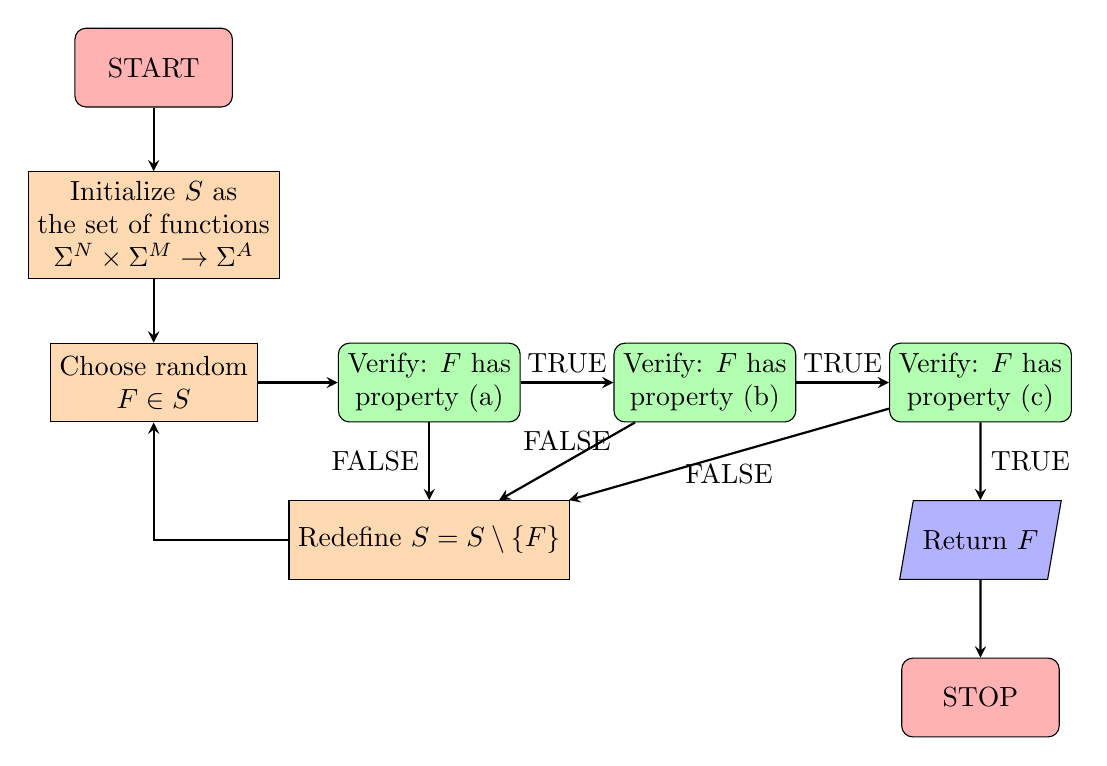
\begin{tikzpicture}[node distance=2cm]
    \node (start) [startstop] {START};
    \node (init) [process, below of=start] {Initialize $S$ as \\the set of functions\\ $\Sigma^N \times \Sigma^M \rightarrow \Sigma^A$ };
    \node (rand) [process, below of=init] {Choose random\\ $F \in S$};
    \node (dec1) [decision, right of=rand, xshift=1.5cm] {Verify: $F$ has\\ property (a)};
    \node (dec2) [decision, right of=dec1, xshift=1.5cm] {Verify: $F$ has\\ property (b)};
    \node (dec3) [decision, right of=dec2, xshift=1.5cm] {Verify: $F$ has\\ property (c)};
    \node (reinit) [process, below of=dec1] {Redefine $S = S \setminus \{F\}$};
    \node (out) [io, below of=dec3] {Return $F$};
    \node (stop) [startstop, below of=out] {STOP};

    \draw [arrow] (start) -- (init);
    \draw [arrow] (init) -- (rand);
    \draw [arrow] (rand) -- (dec1);
    \draw [arrow] (dec1) -- node[anchor=south] {TRUE} (dec2);
    \draw [arrow] (dec2) -- node[anchor=south] {TRUE} (dec3);
    \draw [arrow] (dec3) -- node[anchor=west] {TRUE} (out);
    \draw [arrow] (dec1) -- node[anchor=east] {FALSE} (reinit);
    \draw [arrow] (dec2) -- node[anchor=south] {FALSE} (reinit);
    \draw [arrow] (dec3) -- node[anchor=north] {FALSE} (reinit);
    \draw [arrow] (reinit) -| node[anchor=west] {} (rand);
    \draw [arrow] (out) -- (stop);
\end{tikzpicture}

  \caption{The most na\"ive version of \textsc{AugSolve}, an algorithm which solves a circuit $(N,M,f)$ using the augmented constraints and Lemma \ref{lem:augmented_constraints}}\label{fig:augmented_solve_flowchart}
\end{figure}
However, auxiliary functions which are simultaneously augmented, Ising and neutralizable are exceedingly rare and the space of all auxiliary functions is absurdly large. We therefore need smarter ways of searching for auxiliary functions $F$ if this is to work. Here are some general ideas for improvement:

\begin{idea}[Improvements to \textsc{AugSolve}]\label{idea:improvements_to_AugSolve}$ $
  \begin{enumerate}[(i)]
    \item Instead of choosing $F$ randomly, choose auxiliary functions which are guaranteed to satisfy one of the properties (a), (b) and (c). If possible, this would both drastically shrink the search space $S$ and reduce computation time by removing one of the property verifications. Several versions of this improvement are discussed in the remainder of this section.
    \item Some choices of $F$ are redundant; for example, $F$ and its ``inverse'' $-F$ either both satisfy properties (a) - (c) or both fail to satisfy the same property. Hence, when $F$ is removed from $S$ once might as well remove $-F$ too.
  \end{enumerate}
\end{idea}

\subsubsection{Randomly Sampling Ising Hamiltonians: choosing auxiliary functions which are Ising functions}
Recall that the values of $F$ don't matter -- we care about them only insofar as they allow us to solve the circuit in question. Given this, we can easily find auxiliary functions which are also Ising functions -- simply choose a Hamiltonian $R$ on $X$ and define
\begin{align*}
  F(x,y) = \argmin_{z \in \Sigma^A} H(x,y,z).
\end{align*}
In the case that $|A| = 1$, discussed further in Section \ref{sec:bool_circuits}, this is equivalent to choosing a random hyperplane in $\bR^{N\cup M}$ and using it to partition the cube $\Sigma^{N\cup M}$ into two subsets. This produces the following variation of AugSolve:

\bigskip

\bigg<Algo with [Random Choice] step swapped for \big[Sample Random Ising Hamiltonian from $\bR^P$\big]\bigg>

\bigskip

This easily produces auxiliary functions which satisfy property (b), but there is still lots of redundancy. The Hamiltonian $R$ is entirely parameterized by its coefficients, and small perturbations in these coefficients will produce distinct Hamiltonians without changing the auxiliary function $F$. If it were possible to partition the parameter space $\bR^P$ of $R$ into distinct regions depending on the auxiliary function $F$ induced, then this method on its own might prove quite powerful. As of yet, we do not understand this partition.

\subsubsection{Finding neutralizable Ising functions}

Given a Hamiltonian $R$ on $X$ it is theoretically (if not computationally) straightforward to check whether the auxiliary function $F$ it induces is strongly neutralizable; check whether the ground states associated to a single $x$ are all equal. This requires solving a boolean optimization problem, however; famously difficult.

Instead, consider if for small cardinalities $|A|$, each time we generate a Hamiltonian $R$ we cache the result of the neutralizability check. Over time, we build up a library of auxiliary functions which satisfy both the Ising and neutralizable properties. These can then be ``glued''together to form larger auxiliary functions which are still both neutralizable and Ising.

This method has proven successful even for quite limited libraries of neutralizable Ising functions. An example of this is the ``AND auxiliary'' method. An additional drawback, however, is that the process of desigining a large auxiliary function stitched together from smaller auxiliary functions again involves iterating over a large search space. Designing auxiliary functions with fewer auxiliaries requires a larger library of these smaller functions, and consequently, creates a larger search space.

Another approach for designing neutralizable Ising functions might be to build a pseudo boolean function with the desired properties and reduce it until it is quadratic. This will likely lead to an explosion in the number of auxiliaries, however.

\subsubsection{Reducing the auxiliary function search space using the mixed-integer augmented constraints}

Searching directly for auxiliary functions $F$ such that the $F$-augmented constraints of $(N,M,f)$ are satisfiable is a special type of auxiliary search. However, as the number of auxiliaries grows, no columns are added, so perhaps finding ``augmented-feasible'' auxiliaries is easier than finding typical feasible auxiliary arrays. Even if the full search is still prohibitively expensive, perhaps deductions can be made which reduce the space of possible auxiliary arrays. This could be done by performing Fourier-Motskin on a reduced augmented constraint set for example.

\subsection{Symmetries of Circuits and Systems}
<UNDER CONSTRUCTION>

Let $\Circ(N,M)$ denote the set of all circuits $(N,M,f)$ and $\Ising(X)$ the set of all Ising systems $(X, H)$. We then define the \textbf{Z-space} or \textbf{Zing-space} of $N, M \subset X$ by
\begin{align*}
  \Zing_X(N,M) = \Circ(N,M)\times \Ising(X).
\end{align*}
If $X$ is understood, we often suppress it in the notation and simply write $\Zing(N,M)$. The $\Zing$ stands for ``Zing'' as in the pronunciation of ``Ising'' as ``I-zing''. It also stands for ``Zombiecupcake''.

In this section we develop notions of maps and turn $\Zing(N,M)$ into a category. We are particularly interested in the \emph{symmetries} or \emph{automorphisms} in $\Zing(N,M)$.

\begin{defn}\label{defn:ising-symmetry}
  An \textbf{Ising circuit morphism} or simply an \textbf{Ising map} is a pair of maps $(\alpha_1, \alpha_2)$ with $\alpha_1:\Circ(N,M) \to \Circ(N,M)$ and $\alpha_2:\Ising(X) \to \Ising(X)$ such that
  \begin{align*}
    (X,H) ~ \text{ solves } ~ (N,M,f) ~ \Leftrightarrow~ \alpha_2(X,H) ~ \text{ solves } ~ \alpha_1(N,M,f).
  \end{align*}
  A pair of maps like this is precisely the same as a map on the corresponding product, so we typically denote both maps by $\alpha$ and instead think of $\alpha$ as operating on $\Zing(N,M)$:
  \begin{align*}
    \alpha: \Zing(N,M) \to \Zing(N,M).
  \end{align*}
\end{defn}

Morphisms of Ising circuits is a function on $\Zing(N,M)$ which \emph{preserves the relation of solvability} between circuits and Ising systems.

\begin{example}\label{ex:spinaction}
  Let $\sigma \in \Sigma^X$ be a spin state of $X$. By viewing $\Sigma^X = (\bZ^\times)^{|X|}$, multiplication by $\sigma$ induces a group action of $\Sigma^X$ on itself. We then also have an action functions $f:\Sigma^N \to \Sigma^M$ given by
  \begin{align*}
    (\sigma f)(s) = \sigma_M \cdot f(\sigma_N \cdot s).
  \end{align*}
  This defines a map $\alpha_\sigma: \Circ(N,M) \to \Circ(N,M)$. Correspondingly, if $H$ is an Ising Hamiltonian whose linear terms are denoted $h_i$ and quadratic terms $J_{ij}$ for $i,j \in X$, then by defining $\sigma \cdot H$ to be the Hamiltonian with linear and quadratic terms $h_i'$ and $J_{ij}'$ respectively given
  \begin{align*}
    J_{ij}' = \sigma_i\sigma_j J_{ij}, \hspace{1.5em} h_i' = \sigma_i h_i
  \end{align*}
  we obtain a map $\alpha_\sigma: \Ising(X) \to \Ising(X)$. For any spin $s\in \Sigma^X$ we have
  \begin{align*}
    H(\sigma \cdot s) 
      &= \sum_{i\in X} \sigma_i s_i h_i ~+~ \sum_{i < j} \sigma_{i} s_i \sigma_j s_j J_{ij}  = \sum_{i\in X} (\sigma_i h_i) s_i ~+~ \sum_{i<j} (\sigma_i\sigma_j J_{ij}) s_is_j = (\sigma \cdot H)(s),
  \end{align*}
  hence $(s_N, s_M, s_A)$ minimizes $\sigma \cdot H$ on the input level $\cL(s_N)$ if and only if $(\sigma_N s_N, \sigma_M s_M, \sigma_A s_A)$ minimizes $H$ on the input level $\cL(\sigma_N\cdot s_N)$. This implies that
  \begin{align*}
    (X,H) ~ \text{ solves } ~ (N,M,f) ~\Leftrightarrow ~ \alpha_\sigma (X,H) ~ \text{ solves } ~ \alpha_\sigma (N,M,f).
  \end{align*}
  The actions of $\Sigma^X$ on $\Circ(N,M)$ and $\Ising(X)$ are both referred to as \textbf{spin actions}.
\end{example}

Notice that if $\alpha$ is an Ising symmetry and $\alpha'$ is another Ising symmetry, then $\alpha\circ \alpha'$ is again an Ising symmetry. Since the identity map $\id_{\Zing(N,M)}$ is an Ising morphism, we see that $\Zing(N,M)$ forms a category. Notice also that if $\alpha$ is a bijective Ising symmetry then its inverse $\alpha^{-1}$ is as well, so $\Aut(\Zing(N,M))$ is a group under function composition.

Consider the implications of this setup to the reverse Ising problem. If the group $\Aut(\Zing(N,M))$ were well understood, then every solution $(X,H)$ to $(N,M,f)$ would yield a family of Ising circuits in $\Zing(N,M)$ given by the orbit of $((X,H), (N,M,f))$ under $\Aut(\Zing(N,M))$. This is particularly useful when one isn't interested in solving a specific circuit but rather in understanding the space $\Zing(N,M)$ as a whole for fixed $N$ and $M$, for instance, when designing auxiliary circuits for use with $F$-augmented constraints. The rest of this section is therefore dedicated to developing an understanding of $\Zing(N,M)$.

Let us first imagine enumerating all possible elements of $\Aut(\Zing(N,M))$. One approach might be to write down all bijective maps on $\Circ(N,M)$ and then check which preserve the solvability relation. As a set, $\Circ(N,M)$ is the same as the collection of all functions $f:\Sigma^N \to \Sigma^M$, hence it has size $2^{|N|\cdot 2^{|M|}}$. There are then $\left(2^{|N|\cdot 2^{|M|}}\right)!$ many bijective functions on $\Circ(N,M)$ -- a bit too many to enumerate.

\section{Boolean Circuits and Functions}\label{sec:bool_circuits}
\begin{center}
  <Under construction>
\end{center}

A \textbf{boolean function} is a map $f:\Sigma^N \to \Sigma$. A \textbf{boolean circuit} is an abstract circuit $(N, M, f)$ where $|M| = 1$, and hence where $f$ is a boolean function.

\begin{rmk}[Disambiguation of 0,1 and -1,1 $\Sigma$ representations]\label{rmk:sigma_convention}
  Boolean algebra appears in many disparate fields of math -- game theory, decision theory, coding theory, artificial intelligence and distributed algorithms to name a few -- and hence conventions can vary quite a bit. In particular, the set $\Sigma$ assumes various roles and alternates between $\{-1, 1\}$ and $\{0,1\}$ representations. Results in section \ref{sec:bool_circuits} do not depend on whether $\Sigma = \{0,1\}$ or $\Sigma = \{-1,1\}$, and we will take care to note which definition is currently in use when ambiguity arises. Here is a context-dependent key for swapping between the $\{0,1\}$ and $\{-1,1\}$ representations.
  \begin{itemize}
    \item When $\Sigma$ is regarded as a 2-element set with no additional structure, any bijection between $\{0,1\}$ and $\{-1,1\}$ will suffice.
    \item When $\Sigma$ is regarded as a subset of $\bR$, the change of variables $x \mapsto 2x - 1$ swaps the roles of $0$ and $-1$. This situation arises when considering pseudo-boolean functions $f:\Sigma^N \to \bR$, all of which have unique polynomial representations and hence depend on whether $-1$ or $0$ in use (consider evaluating an Ising Hamiltonian on strings of $0,1$, for instance). It also comes up when one treats a boolean function $f:\Sigma^N \to \Sigma$ as a labeling of the corners of the hypercube $\Sigma^N$, in which case the $\{-1,1\}$ convention is more convenient as it makes the SVM formulas slightly more concise.
    \item When $\Sigma$ is regarded as the unique group $G$ of order 2, there is only identification between $\{0,1\}$ and $\{-1,1\}$ which makes sense: $0 \mapsto 1$ and $1 \mapsto -1$. This is because, $0$ is the identity element when $G$ is regarded as the additive group $\bZ/2\bZ$, but $1$ is the identity when $G$ is regarded as the multiplicative group $\bZ^\times$. Annoyingly, this is distinct from the typical identification, and hence special care must be taken to avoid confusion in situations where the group structure of $\Sigma$ is relevant. The change of variables formula given above can be modified to $x \mapsto 1 - 2x$ if one wishes it to match the group isomorphism.
  \end{itemize}
\end{rmk}

\subsection{Concepts from Boolean Algebra}
\begin{center}
  <Under construction>
\end{center}

\begin{defn}\label{defn:dual-selfdual}
  Let $f:\Sigma^N \to \Sigma$ be a boolean function. The \textbf{dual} of $f$ is a boolean function $f^d$ of the same dimension defined
  \begin{align*}
    f^d(x) = \ol{f(\olx)}.
  \end{align*}
  The \textbf{self-dual} of $f$ is a boolean function $f^{sd}$ of dimension $N+1$ defined
  \begin{align*}
    f^{sd}(x_0, x_1,...,x_n) = \olx_0\cdot f^d(x_1,...,x_n) ~+~ x_0\cdot f(x_1,...,x_n).
  \end{align*}
  The additional bit $x_0$ ``turns $f^d$ and $f$ on and off''.
\end{defn}

\subsection{Ising systems which solve boolean circuits}
\begin{defn}\label{defn:linear_separability}
  Suppose we have a dataset $\cX = (\bfx_1,y_1),...,(\bfx_n,y_n)$ where $\bfx_i$ is a point in $\bR^d$ labeled by $y_i \in \{-1,+1\}$. We say that $\cX$ is \emph{linearly separable} if there exist $\bfw \in \bR^d$ and $b\in \bR$ such that
  \begin{equation}\label{eqn:linear_separability_condition}
    y_i(\bfw^\top \bfx_i - b) > 0.
  \end{equation}
\end{defn}
It turns out that linearly separable labeled datasets correspond precisely to boolean circuits solvable by Ising systems without auxiliaries.
\begin{prop}\label{prop:boolean_ising_svm_equiv}
  Let $(N, M, f)$ be a circuit with one output; i.e., let $|M| = 1$ so that $f$ is a boolean function. There exists an Ising system $(X,H)$ with $X = N \cup M$ which solves $(N,M,f)$ if and only if the set of true vectors $T = f^{-1}(1)$ is linearly separable from the set of false vectors $F = X \setminus F = f^{-1}(-1)$.
\end{prop}
\begin{proof}
  Set $n = |N|$. Under the identifications $\Sigma^N \cong \{-1,1\}^n$ and $M = \Sigma = \{-1,1\}$, we may view $\Sigma^N$ as the vertices of the $n$-dimensional hypercube in $\bR^n$ and the circuit logic $f$ as a labeling of $\Sigma^N$ by $\pm 1$. Denote by $T = f^{-1}(1)$ the set of all vertices in $\Sigma^N$ with label $1$ and by $F = f^{-1}(-1)$ the set of all vertices in $\Sigma^N$ with label $-1$.

  The general form of an Ising Hamiltonian on $X$ is given by
  \begin{equation}\label{eqn:boolean_ising_hamiltonian}
    H(\bfx, y) = \sum_{i = 1}^n h_ix_i ~+~ yh_{n+1} ~+~\sum_{i < j \leq n} J_{ij}\bfx_i\bfx_j ~+~ \sum_{i=1}^nJ_{i,n+1}\bfx_iy.
  \end{equation}
  for some coefficients $h_i$ and $J_{ij}$. The Ising system $(X,H)$ solves the circuit $(N,M,f)$ if and only if the following inequalities are satisfied for all $\bfx \in \Sigma^N$:
  \begin{align*}
    H(\bfx, f(\bfx)) < H(\bfx, -f(\bfx)) 
    ~&\iff~ H(\bfx, -f(\bfx)) - H(\bfx, f(\bfx)) > 0.
  \end{align*}
  Plugging in equation \ref{eqn:boolean_ising_hamiltonian} and canceling terms yields
  \begin{align*}
    H(\bfx, -f(\bfx)) - H(\bfx, f(\bfx)) > 0 
      &\iff \sum_{i=1}^nJ_{i,n+1}\bfx_i(-f(\bfx) - f(\bfx)) ~+~ h_{n+1}(-f(\bfx) - f(\bfx)) > 0 \\
      &\iff f(\bfx)\left(\sum_{i=1}^n -2J_{i,n+1} \bfx_i ~-~ 2h_{n+1}\right) > 0.
  \end{align*}
  This is identical to the linear separability condition \ref{eqn:linear_separability_condition} from Definition \ref{defn:linear_separability} obtained by setting $\bfw = -2J_{\bullet, n+1}$ and $b = -2h_{n+1}$. 
\end{proof}
\begin{rmk}\label{rmk:threshold_functions}
  A boolean function $f:\Sigma^N \to \Sigma$ which produces a linearly separable labeling of $\Sigma^N$ is known as a \textbf{threshold function}. Hence Proposition \ref{prop:boolean_ising_svm_equiv} can be restated as ``a boolean circuit $(N,M,f)$ is solvable if and only if $f$ is a threshold function.'' Counting the number of threshold functions on the $n$-dimensional hypercube is a well studied problem; see OEIS sequence A000609 for instance.
\end{rmk}

Proposition \ref{prop:boolean_ising_svm_equiv} gives us a nice way visualizing Ising solvability. 

\begin{example}\label{ex:AND_XOR_linear_separability}
  Let $N = \{1,2\}$ and $M = \{3\}$. Define two boolean functions $f_1(x_1,x_2) = 4x_1x_2 - 2x_1 - 2x_2 + 1$ and $f_2(x_1,x_2) = -x_1x_2$. Then $(N,M,f_1)$ is the AND circuit and $(N,M,f_2)$ is the XOR circuit, and the labelings they produce on the square $\{-1,1\}^2$ are seen in Figure \ref{fig:AND_XOR_lin_sep}.
  \begin{center}
  \begin{figure}[h]
    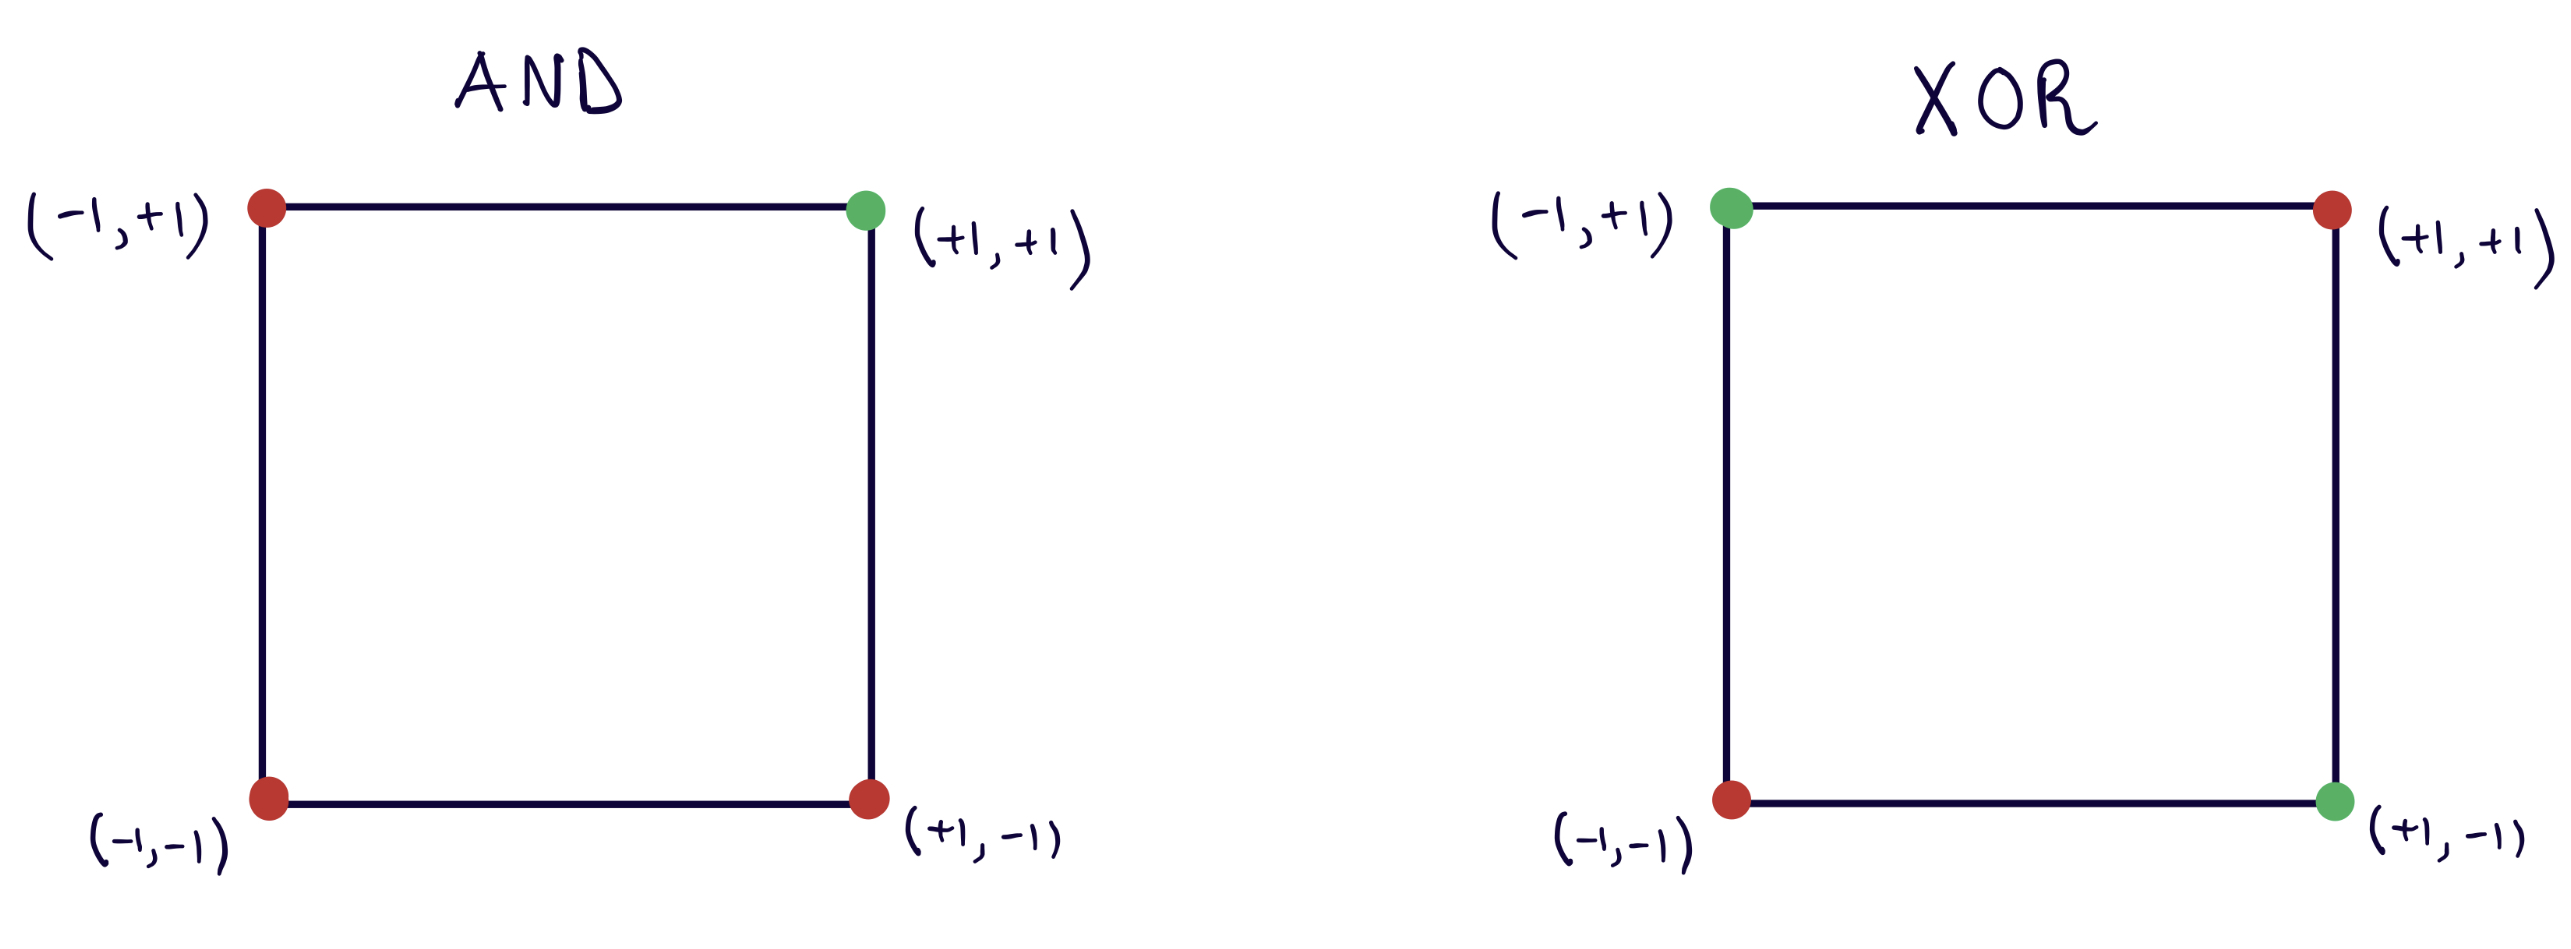
\includegraphics[width=0.95\linewidth]{images/AND_XOR_labeling.jpeg}
    \caption{The labelings produced by AND (left) and XOR (right) where green denotes $+1$ and red denotes $-1$. One can easily draw a line separating the green corner from the three red corners in the AND labeling, but a bit of experimentation should convince the reader that it is impossible to linearly separate the XOR labeling.}
    \label{fig:AND_XOR_lin_sep}
  \end{figure}
  \end{center}
\end{example}

We can use Proposition \ref{prop:boolean_ising_svm_equiv} to easily prove that parity-check circuits are infeasible without auxiliaries.

\begin{prop}\label{prop:parity_checks_are_infeasible}
  Let $N = [n]$, $M = \{n+1\}$ and $f(x_1,...,x_n) = x_1x_2\ldots x_n$. The circuit $(N,M,f)$, called a \textbf{$\bfn$-dimensional parity check}, is infeasible without auxiliaries for $n \geq 2$.
\end{prop}
\begin{proof}
  Consider a hyperplane $\bfw^\top\bfx - b = 0$ in $\bR^n$. If this hyperplane were a linear separation of the $n$-dimensional hypercube labeled by the parity-check circuit, then it would restrict to a linear separation of the $2$-dimensional face $S = \{(x_1,x_2,-1,1,1,...,1) \in \bR^n ~\mid~ x_1,x_2 \in \{-1,+1\}\}$. This is impossible since the parity-check labeling on $S$ is given by $-x_1x_2$. This is exactly the XOR labeling and is hence infeasible.
\end{proof}

\section{Hierarchical Clustering}

A choice of ``auxililary array'' can be thought of as a function $a:\Sigma^N \to \Sigma^A$ which assigns an auxiliary state to each input state. The collection of germs of this function partitions $\Sigma^N$ into subsets of inputs which share the same auxiliary state. To be clear, we're talking about the partition
\begin{align*}
  \{a^{-1}(\alpha)\}_{\alpha \in \Sigma^A}
\end{align*}
of input spin space. If the choice of auxiliary array $a$ makes the Ising circuit feasible, then we say $a$ solves the Ising circuit.

This simple observation motivates a simple question: \emph{can a partition of $\Sigma^N$ be found such that it matches the partition produced by some feasible auxiliary array using only the logic of the Ising circuit?} Producing such a partition is a clustering problem on input spinspace.

\section{Pseudo-boolean optimization and polynomial fitting}
A pseudo boolean function (PBF) is any function $f:\Sigma^N\to \bR$, typically defined so that $\Sigma = \{0,1\}$. It is a well known fact that any such PBF can be uniquely represented by a multilinear polynomial in $n$ variables [pseudo-boolean optimization Boros, Hammer]; that is, a polynomial
\begin{align*}
  g(x_1,...,x_n) = \sum_{S \subset [n]} a_S \prod_{j \in S}x_j
\end{align*}
with $a_S \in \bR$ which equals $f$ pointwise on $\{0,1\}^n$. To be clear, here $S$ iterates over all subsets of $[n] = \{1,...,n\}$.

It is another well-known fact that the optimization of any pseudo-boolean function can be reduced in polynomial time to an optimization problem on a quadratic polynomial. The original method for accomplishing this was first written by Rosenberg, and since then a reputable zoo of alternative algorithms have been introduced. Most methods share the same basic idea: reduce degree $\geq 3$ monomial terms appearing in the polynomial $g$ by introducing auxiliary variables subject to constraints.

<copy Rosenberg algorithm from Boros, Hammer pg 168>

\begin{thm}\label{thm:rosenberg-reduction}
  Let $f$ be a multilinear polynomial in $n$ variables. There exists an algorithm $\textsc{Reduce}$ which produces a multilinear polynomial $g$ in $n + a$ variables such that
  \begin{align*}
    \min_{(\bfx, \bfa) \in \bB^n \times \bB^a} g(\bfx, \bfa) = \min_{\bfx \in \bB^n} f(\bfx)
  \end{align*}
  and if $(\bfx, \bfa) = \arg\min_{(\bfx, \bfa) \in \bB^n \times \bB^a} g(\bfx, \bfa)$ then $\bfx = \arg\min_{\bfx \in \bB^n} f(\bfx).$
\end{thm}
\begin{proof}
  [Boros Hammer Pseudo Boolean Optimization 2002]
\end{proof}
We need a slightly stronger statement however.
\begin{thm}
  Let $f:\Sigma^N \to \Sigma^M$ be a circuit. Then there exists an Ising circuit with auxiliary spins given by Hamiltonian $H$ which solves $f$.
\end{thm}
\begin{proof}
  Fix $G = N \cup M$ and consider the hamming objective function $\operatorname{ham}:\Sigma^N\times \Sigma^M\to \bR$ defined
  \begin{align*}
    \operatorname{ham}(s,t) = d(t, f(s))
  \end{align*}
  where $d(t, f(s))$ is the Hamming distance between $t$ and the correct output $f(s)$. Then there exists some multilinear polynomial $g$ in $|G|$ variables which recovers $\operatorname{ham}$ pointwise. We now apply Rosenberg reduction to $g$ and set $H$ equal to the terminal quadratic polynomial we obtain. All that remains to show is that on any input level $s$ the output which minimizes $H$ is $f(s)$.

  Fix an input $s$ and suppose that the minimizer of $g^k(s, \cdot)$ has output coordinates $f(s)$. To obtain $g^{k+1}$ we replace some pair $x_ix_j$ by $x_{k+1}$ and add the expression $M(x_ix_j - 2x_ix_{k+1} - 2x_jx_{k+1} + 3x_{k+1})$. Observe that this expression is zero if $x_ix_j = x_{k+1}$ and is strictly positive otherwise. It follows that $g^k(\bfx) = g^{k+1}(\bfx, x_{k+1})$ if $x_{k+1} = x_ix_j$ and $g^k(\bfx) < g^{k+1}(\bfx, x_{k+1})$ if $x_{k+1} \neq x_ix_j$. Hence the minimizer of $g^{k+1}$ on input level $s$ also has the correct output coordinates, and inductively, we conclude that $H$ is an Ising Hamiltonian reproducing the circuit $f$.
\end{proof}
\newpage
\bibliographystyle{abbrvnat}
\bibliography{ising}
\end{document}
